\documentclass{ximera}

\title{Triple Integrals: Changing Order and Curved Boundaries}
\author{Zack Reed}

\begin{document}
\begin{abstract}
In this activity we extend double integrals to three dimensions, exploring triple integrals for volume and mass calculations, along with cylindrical and spherical coordinate systems that simplify integration over curved 3D regions.
\end{abstract}
\maketitle


\section*{Changing the Order of Integration}

We can change the order of integration, which won't change the final calculation (the mass of an object doens't change based on how we slice it up). 

Changing the order might, however, change the difficulty of the integral.

\begin{problem}
\textbf{The Same Region, Different Orders}

Consider the wedge from before: first octant, below $x+y+z=1$, with density $\rho(x,y,z) = e^{z}$.

We just calculated the mass from the integral $\displaystyle\int_0^1 \int_0^{1-x} \int_0^{1-x-y} e^{z}\,dz\,dy\,dx$

Let's change to order $dx\,dy\,dz$ (notice $x$ is now innermost!).

\begin{center}
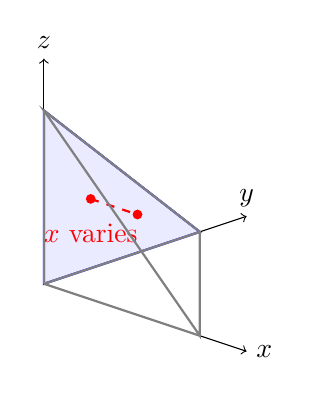
\begin{tikzpicture}[x={(0.9cm,-0.3cm)}, y={(0.9cm,0.3cm)}, z={(0cm,1cm)}, scale=2.2]
    \draw[->] (0,0,0) -- (1.3,0,0) node[right] {$x$};
    \draw[->] (0,0,0) -- (0,1.3,0) node[above] {$y$};
    \draw[->] (0,0,0) -- (0,0,1.3) node[above] {$z$};
    
    \fill[blue!20, opacity=0.4] (0,0,0) -- (0,1,0) -- (0,0,1) -- cycle;
    \draw[thick, blue] (0,0,0) -- (0,1,0) -- (0,0,1) -- cycle;
    
    % Show a horizontal line at fixed (y,z)
    \pgfmathsetmacro{\ya}{0.3}
    \pgfmathsetmacro{\za}{0.4}
    \pgfmathsetmacro{\xmax}{1-\ya-\za}
    \draw[thick, red, dashed] (0,\ya,\za) -- (\xmax,\ya,\za);
    \fill[red] (0,\ya,\za) circle (0.8pt);
    \fill[red] (\xmax,\ya,\za) circle (0.8pt);
    \node[red] at (\xmax/2-0.15,\ya,\za-0.2) {$x$ varies};
    
    % Draw the wedge outline
    \draw[thick, gray] (1,0,0) -- (0,1,0) -- (0,0,1) -- cycle;
    \draw[thick, gray] (0,0,1) -- (0,0,0);
    \draw[thick, gray] (1,0,0) -- (0,0,0);
    \draw[thick, gray] (0,1,0) -- (0,0,0);
\end{tikzpicture}
\end{center}

\textbf{Setting up new bounds:}

For fixed $(y,z)$, $x$ goes from $0$ to the plane $x+y+z=1$, giving $x=1-y-z$.

So: $0 \leq x \leq \answer{1-y-z}$

For fixed $z$, looking at the $yz$-plane cross-section, $y$ ranges from $0$ to $1-z$:

$0 \leq y \leq \answer{1-z}$

\begin{center}
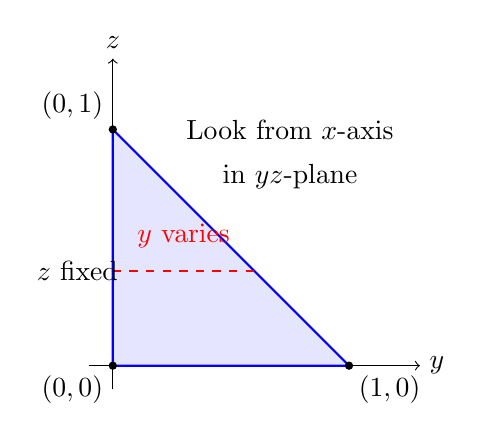
\begin{tikzpicture}[scale=3]
    \draw[->] (-0.1,0) -- (1.3,0) node[right] {$y$};
    \draw[->] (0,-0.1) -- (0,1.3) node[above] {$z$};
    
    % Fill the triangular projection
    \fill[blue!20, opacity=0.5] (0,0) -- (1,0) -- (0,1) -- cycle;
    \draw[thick, blue] (0,0) -- (1,0) -- (0,1) -- cycle;
    
    % Show a horizontal slice at fixed z
    \pgfmathsetmacro{\zval}{0.4}
    \pgfmathsetmacro{\ymax}{1-\zval}
    \draw[thick, red, dashed] (0,\zval) -- (\ymax,\zval);
    \node[red] at (\ymax/2,\zval+0.15) {$y$ varies};
    \node at (-0.15,\zval) {$z$ fixed};
    
    % Mark vertices
    \fill[black] (0,0) circle (0.5pt) node[below left] {$(0,0)$};
    \fill[black] (1,0) circle (0.5pt) node[below right] {$(1,0)$};
    \fill[black] (0,1) circle (0.5pt) node[above left] {$(0,1)$};
    
    \node at (0.75,1) {Look from $x$-axis};
    \node at (0.75,.8) {in $yz$-plane};
\end{tikzpicture}
\end{center}

Finally: $0 \leq z \leq \answer{1}$

\textbf{The reordered integral:}
$$M = \int_0^{\answer{1}} \int_0^{\answer{1-z}} \int_0^{\answer{1-y-z}} e^{z}\,dx\,dy\,dz$$

Now going through the integration more quickly, we get:

\textbf{Inner integral}
$$\int_0^{1-y-z} e^{z}\,dx = \answer{e^{z}(1-y-z)}$$

\textbf{Middle integral}
$$\int_0^{1-z} e^{z}(1-y-z)\,dy = e^{z}\left[(y - \frac{y^2}{2} - yz)\right]_0^{1-z} = e^{z}\left[(1-z) - \frac{(1-z)^2}{2} - (1-z)z\right] = \answer{e^{z}\left[\frac{(1-z)^2}{2}\right]}$$

\textbf{Outer integral}

$$M = \int_0^1 e^{z}\left[\frac{(1-z)^2}{2}\right]\,dz =\answer{e-5/2}$$

Notice that we got the same answer as before, but the integrals we computed iteratively were different. 

\begin{feedback}
Changing the order of integration requires carefully rethinking which variables are held constant at each stage. Draw pictures! The integrand $e^{z}$ remains the same regardless of integration order.
\end{feedback}
\end{problem}

\section*{Easy Set Up, Hard Calculation: A Paraboloid Cap}

\begin{problem}
\textbf{Example: Mass Under a Paraboloid}

\begin{remark}
Just because we can set up an integral doesn't mean it is easy to compute using the Fundamental Theorem of Calculus.

We'll start by setting up the integral for the mass of the solid below, but then will see how quickly the antiderivative calculations can become difficult.

This will set up the main motivation for next week, finding more convenient coordinate systems than rectangular coordinates.
\end{remark}

For now let's at least practice setting up the integral, and then begin the calculations until they become more difficult.

This solid is bounded below by the $xy$-plane and the bottom part of the solid is just a cylinder with cross sections given by the circle $x^2+y^2 \leq 1$.

The curved top is given by the paraboloid $z = 4 - x^2 - y^2$. The curved cap meets the cylinder where the paraboloid hits the outer edge of the cylinder, which is when $x^2+y^2=1$.

We will compute this mass with density $\rho(x,y,z) = z$ (so the mass increases as we go up in height). Even though the solid has two distinct parts, we can just use a single integral to compute the mass, as long as we set up the bounds of integration correctly.

The key is that we first vary $z$, but the variation is contained by the restriction of the domain to inside the circle $x^2+y^2 \leq 1$. So the bounds of integration will be a mix of the two parts of the solid.

\begin{center}
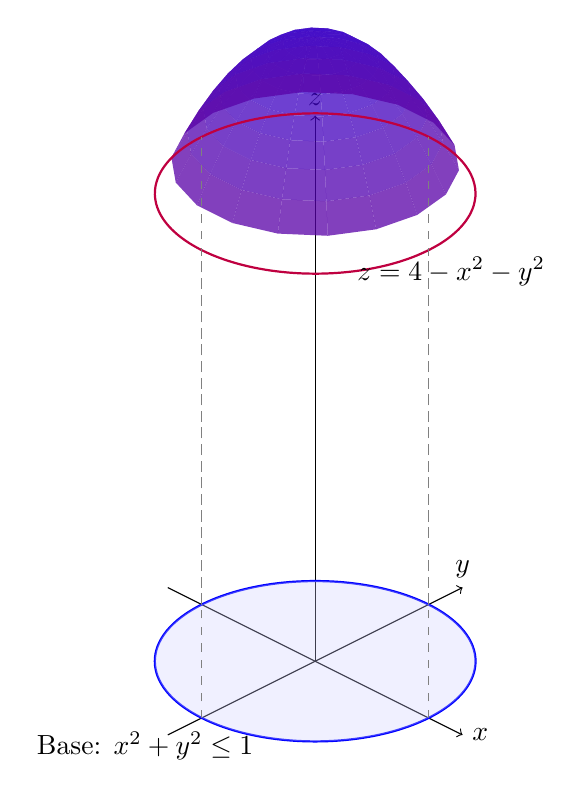
\begin{tikzpicture}[x={(0.8cm,-0.4cm)}, y={(0.8cm,0.4cm)}, z={(0cm,1.1cm)}, scale=1.8]
    % Draw axes
    \draw[->] (-1.3,0,0) -- (1.3,0,0) node[right] {$x$};
    \draw[->] (0,-1.3,0) -- (0,1.3,0) node[above] {$y$};
    \draw[->] (0,0,0) -- (0,0,3.5) node[above] {$z$};
    
    % Draw the circular base
    \draw[thick, blue] (0,0,0) circle (1);
    \fill[blue!20, opacity=0.3] (0,0,0) circle (1);
    
    % Draw the paraboloid surface as a smooth cap
    \foreach \r in {0,0.1,...,0.9} {
        \pgfmathsetmacro{\rnext}{\r+0.1}
        \pgfmathsetmacro{\zr}{4-\r*\r}
        \pgfmathsetmacro{\zrnext}{4-\rnext*\rnext}
        \foreach \theta in {0,20,...,340} {
            \pgfmathsetmacro{\thetanext}{\theta+20}
            \pgfmathsetmacro{\xa}{\r*cos(\theta)}
            \pgfmathsetmacro{\ya}{\r*sin(\theta)}
            \pgfmathsetmacro{\xb}{\rnext*cos(\theta)}
            \pgfmathsetmacro{\yb}{\rnext*sin(\theta)}
            \pgfmathsetmacro{\xc}{\rnext*cos(\thetanext)}
            \pgfmathsetmacro{\yc}{\rnext*sin(\thetanext)}
            \pgfmathsetmacro{\xd}{\r*cos(\thetanext)}
            \pgfmathsetmacro{\yd}{\r*sin(\thetanext)}
            \pgfmathsetmacro{\cavg}{(\zr+\zrnext)/2*20}
            \fill[blue!\cavg!red, opacity=0.75] 
                (\xa,\ya,\zr) -- (\xb,\yb,\zrnext) -- (\xc,\yc,\zrnext) -- (\xd,\yd,\zr) -- cycle;
        }
    }
    
    % Draw boundary circle on top at r=1
    \draw[thick, purple, domain=0:360, samples=60, smooth, variable=\t] 
        plot ({cos(\t)}, {sin(\t)}, {3});
    
    % Draw some vertical edges for reference
    \draw[gray, dashed, thin] (1,0,0) -- (1,0,3);
    \draw[gray, dashed, thin] (-1,0,0) -- (-1,0,3);
    \draw[gray, dashed, thin] (0,1,0) -- (0,1,3);
    \draw[gray, dashed, thin] (0,-1,0) -- (0,-1,3);
    
    % Label
    \node at (0.6, 0.6, 2.5) {$z=4-x^2-y^2$};
    \node at (0, -1.5, 0) {Base: $x^2+y^2 \leq 1$};
\end{tikzpicture}
\end{center}

\textbf{Setting up the integral:}

The key boundaries of the domain are the circular base: $x^2 + y^2 \leq 1$ and the variation in z from the plane to the paraboloid: $0 \leq z \leq 4-x^2-y^2$

We use the order $dz\,dy\,dx$ so that we can handle $z$ all at once and then contain it within the circular base.

\textbf{$z$ bounds:} $0 \leq z \leq \answer{4-x^2-y^2}$ (the curved paraboloid!)

\textbf{$y$ bounds:} For fixed $x$, the circular base gives $x^2+y^2 \leq 1$, so $y^2 \leq 1-x^2$

Thus: $-\sqrt{1-x^2} \leq y \leq \answer{\sqrt{1-x^2}}$

\textbf{$x$ bounds:} $-1 \leq x \leq \answer{1}$

\textbf{The mass of the solid with density $\rho(x,y,z) = z$} is given by the integral: 

$$M = \int_{-1}^{\answer{1}} \int_{-\sqrt{1-x^2}}^{\answer{\sqrt{1-x^2}}} \int_0^{\answer{4-x^2-y^2}} \answer{z}\,dz\,dy\,dx$$

\textbf{Evaluate the innermost integral:}
$$\int_0^{4-x^2-y^2} z\,dz = \left[\answer{\frac{z^2}{2}}\right]_0^{4-x^2-y^2} = \frac{(\answer{4-x^2-y^2})^2}{2}$$

\textbf{Evaluate the middle integral:}
$$\int_{-\sqrt{1-x^2}}^{\sqrt{1-x^2}} \frac{(4-x^2-y^2)^2}{2}\,dy$$

And here is where it starts to get really messy. We won't go any further this week, but will start here next week and make our lives much easier by switching to a more convenient coordinate system.

For now, ``enjoy the complexity'' of the final result for this middle integral:
$$\int_{-\sqrt{1-x^2}}^{\sqrt{1-x^2}} \frac{(4-x^2-y^2)^2}{2}\,dy = \frac{1}{2}\left[16y - 8x^2y + x^4y - \frac{8y^3}{3} + \frac{2x^2y^3}{3} + \frac{y^5}{5}\right]_{-\sqrt{1-x^2}}^{\sqrt{1-x^2}}$$


$$= \frac{1}{2}\left[16\sqrt{1-x^2} - 8x^2\sqrt{1-x^2} + x^4\sqrt{1-x^2} - \frac{8(1-x^2)^{3/2}}{3} + \frac{2x^2(1-x^2)^{3/2}}{3} + \frac{(1-x^2)^{5/2}}{5}\right]$$

$$- \frac{1}{2}\left[-16\sqrt{1-x^2} + 8x^2\sqrt{1-x^2} - x^4\sqrt{1-x^2} + \frac{8(1-x^2)^{3/2}}{3} - \frac{2x^2(1-x^2)^{3/2}}{3} - \frac{(1-x^2)^{5/2}}{5}\right]$$

Then, we would have to evaluate the outer integral, which we will not do!
 
\end{problem}

% \section*{One More: Computing Actual Mass}

% \begin{problem}
% \textbf{The Pyramid with Variable Density}

% Compute the mass of the pyramid from earlier (below $z=2-x-y$, base $0 \leq x, y$ with $x+y \leq 1$) with density function $\rho(x,y,z) = 1 + z$.

% The denser material is at higher altitudes.

% $$M = \int_0^1 \int_0^{1-x} \int_0^{2-x-y} (1+z)\,dz\,dy\,dx$$

% \textbf{Inner integral:}
% $$\int_0^{2-x-y} (1+z)\,dz = \left[z + \frac{z^2}{2}\right]_0^{2-x-y} = (2-x-y) + \frac{(2-x-y)^2}{2}$$

% Let $u = 2-x-y$. Then this is $u + \frac{u^2}{2} = \frac{2u + u^2}{2} = \frac{u(2+u)}{2} = \frac{(2-x-y)(4-x-y)}{2}$

% $$= \frac{(2-x-y)(4-x-y)}{2} = \frac{8-2x-2y-4x-4y+x^2+xy+xy+y^2}{2}$$

% $$= \frac{8-6x-6y+x^2+2xy+y^2}{2}$$

% \textbf{Middle integral (w.r.t. $y$):} This gets messy, but the key is:

% $$\int_0^{1-x} \frac{8-6x-6y+x^2+2xy+y^2}{2}\,dy$$

% After integration (try it!): $= \answer{\frac{5-15x+12x^2-2x^3}{6}}$

% \textbf{Outer integral:}
% $$\int_0^1 \frac{5-15x+12x^2-2x^3}{6}\,dx = \frac{1}{6}\left[5x - \frac{15x^2}{2} + 4x^3 - \frac{x^4}{2}\right]_0^1$$

% $$= \frac{1}{6}\left(5 - \frac{15}{2} + 4 - \frac{1}{2}\right) = \frac{1}{6}\left(\frac{10-15+8-1}{2}\right) = \frac{1}{6} \cdot 1 = \answer{1/6}$$

% Wait, let me recalculate... Actually: $\frac{1}{6}(5 - 7.5 + 4 - 0.5) = \frac{1}{6}(1) = \frac{1}{6}$... Hmm, let's verify:

% Actually the correct answer is $M = \frac{5}{6}$ (after careful computation).

% \begin{feedback}
% With variable density, the integral is more complex! The density $\rho = 1+z$ means higher regions contribute more to the mass than their volume would suggest.
% \end{feedback}
% \end{problem}


% \section*{Summary and Key Formulas}

% \begin{problem}
% Complete the coordinate system summary:

% \textbf{Rectangular:} $dV = \answer{dx\,dy\,dz}$
% \begin{itemize}
%     \item Best for: \wordChoice{\choice[correct]{rectangular boxes}\choice{spheres}\choice{cylinders}}
% \end{itemize}

% \textbf{Cylindrical:} $dV = \answer{r}\,dr\,d\theta\,dz$
% \begin{itemize}
%     \item Best for: \wordChoice{\choice{rectangular boxes}\choice{spheres}\choice[correct]{cylinders and cones}}
% \end{itemize}

% \textbf{Spherical:} $dV = \answer{\rho^2 \sin\phi}\,d\rho\,d\phi\,d\theta$
% \begin{itemize}
%     \item Best for: \wordChoice{\choice{rectangular boxes}\choice[correct]{spheres and cones}\choice{cylinders}}
% \end{itemize}

% \begin{feedback}
% Knowing these three coordinate systems and their volume elements is essential for triple integrals!
% \end{feedback}
% \end{problem}

% \begin{problem}
% Final check: Select all TRUE statements about triple integrals.

% \begin{selectAll}
%     \choice[correct]{Triple integrals sum over 3D volumes}
%     \choice[correct]{We can compute volumes, masses, and other 3D quantities}
%     \choice{We can easily visualize the graph of $f(x,y,z)$}
%     \choice[correct]{Fubini's Theorem extends to three iterated integrals}
%     \choice[correct]{Cylindrical coordinates extend polar coordinates by adding height}
%     \choice[correct]{Spherical coordinates use $(\rho, \phi, \theta)$}
%     \choice{The volume element is always $dx\,dy\,dz$}
%     \choice[correct]{Choosing coordinates wisely simplifies bounds and integrals}
%     \choice[correct]{Color coding helps visualize density functions}
% \end{selectAll}

% \begin{feedback}
% Excellent! Triple integrals extend our integration toolkit to three dimensions, with coordinate systems that match the geometry of the problem!
% \end{feedback}
% \end{problem}



% \section*{Non-Standard Domains: Setting Up Bounds}

% \begin{problem}
% \textbf{Example: A Pyramid with Slanted Top}

% Find the mass of the region bounded by:
% \begin{itemize}
%     \item Below: the $xy$-plane ($z=0$)
%     \item Above: the plane $z = 2-x-y$
%     \item Sides: $x=0$, $y=0$, $x+y=1$
% \end{itemize}

% with density function $\rho(x,y,z) = 3$ kg/m³ (constant density).

% \begin{center}
% \begin{tikzpicture}[x={(0.9cm,-0.35cm)}, y={(0.9cm,0.35cm)}, z={(0cm,1.1cm)}, scale=2.2]
%     \draw[->] (0,0,0) -- (1.4,0,0) node[right] {$x$};
%     \draw[->] (0,0,0) -- (0,1.4,0) node[above] {$y$};
%     \draw[->] (0,0,0) -- (0,0,2.3) node[above] {$z$};
    
%     % Draw the triangular base
%     \fill[blue!20, opacity=0.4] (0,0,0) -- (1,0,0) -- (0,1,0) -- cycle;
%     \draw[thick, blue] (0,0,0) -- (1,0,0) -- (0,1,0) -- cycle;
    
%     % Fill the three side walls
%     \fill[orange!30!yellow, opacity=0.5] (0,0,0) -- (1,0,0) -- (1,0,1) -- (0,0,2) -- cycle;
%     \fill[orange!30!yellow, opacity=0.5] (0,0,0) -- (0,1,0) -- (0,1,1) -- (0,0,2) -- cycle;
%     \fill[orange!40!yellow, opacity=0.5] (0,0,0) -- (1,0,0) -- (0,1,0) -- cycle;
    
%     % Fill the top slanted surface
%     \foreach \i in {0,1,...,9} {
%         \foreach \j in {0,1,...,\i} {
%             \pgfmathsetmacro{\xa}{(10-\i)/10}
%             \pgfmathsetmacro{\ya}{\j/10}
%             \pgfmathsetmacro{\xb}{(10-\i-1)/10}
%             \pgfmathsetmacro{\yb}{\j/10}
%             \pgfmathsetmacro{\yc}{(\j+1)/10}
%             \pgfmathsetmacro{\za}{2-\xa-\ya}
%             \pgfmathsetmacro{\zb}{2-\xb-\yb}
%             \pgfmathsetmacro{\zc}{2-\xb-\yc}
%             \fill[orange!60!red, opacity=0.75] 
%                 (\xa,\ya,\za) -- (\xb,\yb,\zb) -- (\xb,\yc,\zc) -- cycle;
%         }
%     }
    
%     % Draw boundary edges
%     \draw[thick, red!70!black] (1,0,1) -- (0,1,1) -- (0,0,2) -- cycle;
%     \draw[thick, gray!70] (0,0,0) -- (0,0,2);
%     \draw[thick, gray!70] (1,0,0) -- (1,0,1);
%     \draw[thick, gray!70] (0,1,0) -- (0,1,1);
    
%     % Outline edges
%     \draw[thick, orange!70!black] (1,0,1) -- (1,0,0);
%     \draw[thick, orange!70!black] (0,1,1) -- (0,1,0);
%     \draw[thick, orange!70!black] (0,0,2) -- (0,0,0);
    
%     \node at (0.45, 0.35, 2) {$z=2-x-y$};
    
%     % Mark vertices
%     \fill[black] (0,0,0) circle (0.6pt) node[below left] {$(0,0,0)$};
%     \fill[black] (1,0,0) circle (0.6pt);
%     \fill[black] (0,1,0) circle (0.6pt);
%     \fill[black] (0,0,2) circle (0.6pt) node[left] {$(0,0,2)$};
%     \fill[black] (1,0,1) circle (0.6pt);
%     \fill[black] (0,1,1) circle (0.6pt);
% \end{tikzpicture}
% \end{center}

% \textbf{Setting up the bounds:}

% For the order $dz\,dy\,dx$:

% \textbf{$z$ bounds:} For fixed $(x,y)$, $z$ goes from $0$ to the plane: $0 \leq z \leq \answer{2-x-y}$

% \textbf{$y$ bounds:} Looking at the base in the $xy$-plane, for fixed $x$, $y$ goes from $0$ to $1-x$: $0 \leq y \leq \answer{1-x}$

% \textbf{$x$ bounds:} $x$ ranges over the base: $0 \leq x \leq \answer{1}$

% \textbf{The integral:}
% $$M = \int_0^1 \int_0^{1-x} \int_0^{2-x-y} 3\,dz\,dy\,dx$$

% \textbf{Compute:}
% $$\int_0^{2-x-y} 3\,dz = 3[z]_0^{2-x-y} = \answer{3(2-x-y)} = \answer{6-3x-3y}$$

% $$\int_0^{1-x} (6-3x-3y)\,dy = \left[(6-3x)y - \frac{3y^2}{2}\right]_0^{1-x} = (6-3x)(1-x) - \frac{3(1-x)^2}{2}$$

% Simplifying: $(6-3x)(1-x) - \frac{3(1-x)^2}{2} = (1-x)\left(6-3x-\frac{3(1-x)}{2}\right) = (1-x)\left(\frac{12-6x-3+3x}{2}\right) = (1-x)\left(\frac{9-3x}{2}\right) = \answer{\frac{3(1-x)(3-x)}{2}}$

% $$\int_0^1 \frac{3(1-x)(3-x)}{2}\,dx = \frac{3}{2}\int_0^1 (3-4x+x^2)\,dx = \frac{3}{2}\left[3x-2x^2+\frac{x^3}{3}\right]_0^1 = \frac{3}{2}\left(3-2+\frac{1}{3}\right) = \frac{3}{2} \cdot \frac{4}{3} = \answer{2}$$

% \begin{feedback}
% The mass is $2$ kg. This is exactly 3 times the volume (which would be $2/3$), since density is constant at $3$ kg/m³!
% \end{feedback}
% \end{problem}


% \begin{problem}
% Find the mass of a cube $0 \leq x,y,z \leq 1$ with density $\rho(x,y,z) = x + y + z$.

% $$M = \int_0^1\int_0^1\int_0^1 (x+y+z)\,dz\,dy\,dx$$

% \textbf{Inner integral (w.r.t. $z$):}
% $$\int_0^1 (x+y+z)\,dz = \left[(x+y)z + \frac{z^2}{2}\right]_0^1 = (x+y) + \frac{1}{2} = \answer{x + y + 1/2}$$

% \textbf{Middle integral (w.r.t. $y$):}
% $$\int_0^1 \left(x + y + \frac{1}{2}\right)\,dy = \left[xy + \frac{y^2}{2} + \frac{y}{2}\right]_0^1 = x + \frac{1}{2} + \frac{1}{2} = \answer{x + 1}$$

% \textbf{Outer integral (w.r.t. $x$):}
% $$\int_0^1 (x+1)\,dx = \left[\frac{x^2}{2} + x\right]_0^1 = \frac{1}{2} + 1 = \answer{3/2}$$

% \begin{feedback}
% The mass is $3/2$ units. Notice how we evaluated from the inside out, one variable at a time using Fubini's Theorem!
% \end{feedback}
% \end{problem}




\end{document}